\phantomsection\numberedsection{RF6.3 Modificar Atributo}

\subsection*{Descripción}
Los usuarios pueden modificar los atributos de usuario ya existentes en la cuenta.
\vspace{0.15cm}

\textbf{Pre-condición}\par
El usuario ha iniciado sesión en su cuenta en Mini PIM, tiene acceso a la sección de gestión de atributos y hay al menos un atributo de usuario creado.\par
\vspace{0.15cm}

\textbf{Post-condición}
\begin{itemize}
    \item Caso de éxito: El atributo es modificado y reflejado en la base de datos, asociado al usuario correspondiente.
    \item Caso mínimo: El sistema notifica al usuario el resultado de la acción modificar atributo; exitosa o fallida.
\end{itemize}

\textbf{Prioridad: }
Alta
\vspace{0.15cm}

\textbf{Autor: }
Pablo Ortega y Diego Sicre.\par
\vspace{0.15cm}

\textbf{Control de cambios: }
\begin{itemize}
    \item Versión 1: Definición del caso de uso.
\end{itemize}

\numberedsubsection{Escenario principal}
\begin{enumerate}
    \item El usuario selecciona el atributo que quiere modificar haciendo doble clic en el \textit{GridAtributos}.
    \item El usuario hace doble clic en el \textit{GridAtributos}.
    \item El sistema muestra un desplegable en el \textit{tipo de datos} y permite escribir en la columna de \textit{nombre}.
    \item El usuario modifica los datos solicitados:
    \begin{itemize}
        \item Si selecciona Texto como tipo de dato, el sistema establece un límite de 250 caracteres para el valor.
    \end{itemize}
    \item El usuario confirma la modificación del atributo haciendo \textit{enter}.
    \item El sistema verifica que:
    \begin{itemize}
        \item El nombre del atributo y el tipo de dato son válidos y cumplen las restricciones establecidas.
    \end{itemize}
    \item El sistema almacena el atributo en la base de datos, asociado al usuario.
    \item El sistema muestra al usuario un mensaje confirmando que el atributo ha sido modificado con éxito
\end{enumerate}

\numberedsubsection{Escenarios alternativos}
\begin{description}
    \item[2.a] El usuario selecciona un tipo de dato incorrecto o no soportado por el sistema.
    \begin{enumerate}
        \item[2.a.1] El sistema muestra un mensaje de error indicando que el tipo de dato seleccionado no es válido y permite al usuario realizar los ajustes necesarios.
    \end{enumerate}

    \item[3.a] El sistema detecta un error en la validación del nombre o tipo de dato del atributo.
    \begin{enumerate}
        \item[3.a.1] El sistema notifica al usuario el error específico en el campo afectado y permite editar los datos.
    \end{enumerate}
\end{description}

\numberedsubsection{Casos de Prueba}
\underline{Escenario: Principal}\par
\vspace{0.15cm}
\textbf{Dado} que el usuario ha iniciado sesión en su cuenta en Mini PIM,\par
\textbf{Y} se encuentra en la sección de atributos,\par
\textbf{Y} selecciona un atributo,
\textbf{Cuando} hace doble clic en el atributo,\par
\textbf{E} introduce un nombre y selecciona un tipo de dato válido,\par
\textbf{Y} confirma la modificación,\par
\textbf{Entonces} el sistema almacena el atributo en la base de datos y lo muestra en \textit{GridAtributos}.\par
\vspace{0.20cm}

\underline{Escenario: Alternativo 2.a}\par
\vspace{0.15cm}
\textbf{Dado} que el usuario intenta seleccionar un tipo de dato no soportado,\par
\textbf{Cuando} confirma la modificación del atributo,\par
\textbf{Entonces} el sistema muestra un mensaje de error y permite al usuario corregir la selección del tipo de dato.\par
\vspace{0.20cm}

\underline{Escenario: Alternativo 3.a}\par
\vspace{0.15cm}
\textbf{Dado} que el usuario ha dejado el nombre del atributo vacío,\par
\textbf{Cuando} intenta confirmar la creación,\par
\textbf{Entonces} el sistema muestra un mensaje de error indicando el campo faltante y permite al usuario corregirlo.\par
\vspace{0.20cm}


\numberedsubsection{Bocetos}
\begin{figure}[H]
    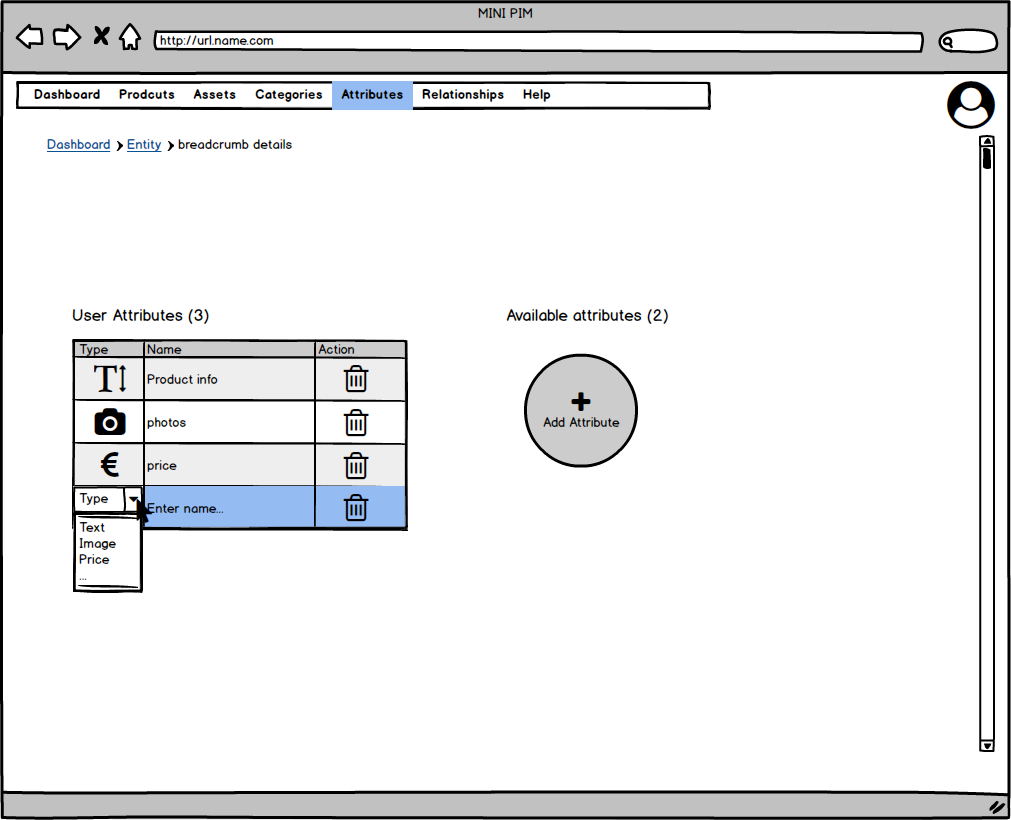
\includegraphics[width=1\linewidth]{mockups/RF6.3Modificar_AtributoV2.png}
    \caption{Apartado Atributos tras clicar dos veces en el atributo que se desea editar}
   \end{figure}
\vspace{1.0cm}

\newpage %Inicia en una nueva página otro caso de uso